% ВАЖНО
% Не меняйте ничего в этом файле. А если меняете, то делайте это в этом проекте:
% https://github.com/kib-courses/latex_templates
% Для пользовательских настроек есть файл ./header/user.tex
\documentclass{beamer}
\usetheme{metropolis} 
\usecolortheme{rose}

\hypersetup{unicode=true}
\usepackage{tikz}

\usepackage{xcolor}
\usepackage[utf8]{inputenc}
\usepackage{hyphenat}
\usepackage[russian,english]{babel}          % Use metropolis theme
\usepackage{wrapfig}

\usepackage[normalem]{ulem}  % для зачекивания текста

\usepackage{caption}
\captionsetup[figure]{name=Рисунок }
\newcommand{\рис}[1]{рис.\ref{#1}}
\newcommand{\Рис}[1]{Рис.\ref{#1}}


\captionsetup[table]{name=Таблица~№}
\newcommand{\таблицa}[1]{таблица~№\ref{#1}} % именительный падеж
\newcommand{\таблицы}[1]{таблицы~№\ref{#1}} % родительный падеж
\newcommand{\таблице}[1]{таблице~№\ref{#1}} % дательный и предложный падеж
\newcommand{\таблицу}[1]{таблицу~№\ref{#1}} % винительный падеж
\newcommand{\таблицей}[1]{таблицей~№\ref{#1}} % творительный падеж 
\newcommand{\Таблицa}[1]{Таблица~№\ref{#1}} % именительный падеж
\newcommand{\Таблицы}[1]{Таблицы~№\ref{#1}} % родительный падеж
\newcommand{\Таблице}[1]{Таблице~№\ref{#1}} % дательный и предложный падеж
\newcommand{\Таблицу}[1]{Таблицу~№\ref{#1}} % винительный падеж
\newcommand{\Таблицей}[1]{Таблицей~№\ref{#1}} % творительный падеж 

\setbeamertemplate{footline}[frame number] % указывает на каждой странице общее количество страниц

% Указывайте все новые термины в \termdef команде. А уже известные ранее или из других курсов в \term
\newcommand{\termdef}[1]{\textbf{\textit{#1}}}
\newcommand{\term}{\textit}

% Диалог с аудиторией.
\newcommand{\auditorium}[1]{\textcolor{red}{\textbf{#1}}}

\let\OLDhref\href
\renewcommand{\href}[2]{\textcolor{blue}{\OLDhref{#1}{#2}}}

% \setbeameroption{show notes}
% \usepackage{listings}             % Include the listings-package
% \usepackage{minted}

\usepackage{CJKutf8}

\title{Лекция 2. Классификация: основные понятия. Пример алгоритма классификации: Random Forest}
% \date{\today}
\date{24 сентября 2019}
\author{Павел Владимирович Слипенчук}
\institute{Москва, МГТУ им.Бауманка,\\ каф.ИУ-8, КИБ}
% \titlegraphic{\includegraphics[width=2cm]{logo_ur.jpg}}
\titlegraphic{\small \href{https://github.com/kib-courses/dsis}{Data Science для решения задач информационной безопасности}}

\begin{document}
  \maketitle
    
  \begin{frame}{План лекции}
    \begin{enumerate}
	\item \nameref{section:classification_defs}
	\item \nameref{section:precision_recall_defs}
	\item \nameref{section:tree_forest}
	\item \nameref{section:random_tree_building}
	\item \nameref{section:random_forest}
	\end{enumerate}
 \end{frame}
    
  \section{Признак. Вектор признаков Классы. Обучающая и тестовая выборки. Задача классификации, классификатор(оценщик)}\label{section:classification_defs}
  
  \begin{frame}{Признак, вектор, класс}
    \termdef{Признак} $x_i$-- определенное значение. Категориальное, сравнимое, или числовое: целочисленное, булевое, или дробное.
    
    \termdef{Вектор признаков} $\bold x = (x_1, x_2, ... x_n)$ -- вектор, каждое значение которого является \term{признаком}. 
  	
  	\termdef{Класс} (метка) $y$ -- значение (как правило целочисленное), присваиваемое какому-либо вектору признаков: $ y \mapsto \bold x$
  	
  	\auditorium{А в чем физический смысл?}
  \end{frame}
  
  \begin{frame}{Пример}\label{frame:class_feature_vector_example}
  \begin{itemize}
  	 \item $x_1$ -- сумма транзакции [в рублях]
  	 \item $x_2$ -- возраст клиента [в годах]
  	 \item $x_3$ -- пол клиента [булевый: 1 -- мужской, 0 -- женский]
  	 \item $x_4$ -- MCC код\footnote{\termdef{Merchant Category Code} -- номер деятельности компании при осуществлении безналичной оплаты. Например \textbf{1731} означает оплату за электроэнергию, \textbf{3137} -- покупка авиабилетов, \textbf{4121} -- такси}
  	 \item  $y=1$ -- операция мошенническая (фродовая);  $y=0$ -- легитимная.
  \end{itemize}
  \begin{center}\small \begin{tabular}{ l l }
  	$0 \mapsto (3234, 25, 1, 1731) $ &  $0 \mapsto (2540, 55, 0, 1731)$ \\
  	$1 \mapsto (18400, 45, 0, 3137)$ & $0 \mapsto (2540, 55, 0, 1731)$  \\
  	$1 \mapsto (903, 19, 0, 4121)$  & $0 \mapsto (1875, 45, 0, 4121)$  \\
  	$0 \mapsto (854, 21, 1, 4121)$  & $1 \mapsto (702, 21, 0, 4121)$  \\
  	$1 \mapsto (903, 19, 0, 4121)$  & $0 \mapsto (1875, 45, 0, 4121)$  \\
  	$0 \mapsto (28400, 41, 1, 3137)$ & $0 \mapsto (25040, 55, 0, 1731)$  \\
  \end{tabular}\end{center}
  \end{frame}
  
  \begin{frame}
   \begin{block}{Замечание}
	  В отличие от таблицы, представленной на слайде №\ref{frame:class_feature_vector_example},
	  в данных на реальных задачах \term{вектор признаков} может состоять из $~200$ и более признаков:
	  $\bold x = (x_1, x_2, ..., x_{200}, ...)$
  \end{block}
   \end{frame}

  \begin{frame}
\begin{block}{Замечание}
	Иногда можно встретить ещё два понятия: \term{характеристика} и \term{контрибутор}.
	
	\termdef{Характеристика} -- это какая-либо информация из которой можно получить один
	или более признаков.
	
	\termdef{Контрибутор} (контрибьютер) -- это совокупность признаков (возможно один),
	который вносит определённый вклад в скоринговую модель. 
	
	Однако можно считать эти термины устаревшими, так как
	\term{Feature Extraction} ввело понятие \term{<<сырые данные>>} (raw data)
	и убило понятие характеристика; 
	а ансамбли сделали ненужным термин контрибутор.
\end{block}
\end{frame}

  
  \begin{frame}{Функция высшего порядка}
  \termdef{Функция высшего порядка} -- это функция, принимающая в качестве аргументов хотя бы одну другую функцию и/или возвращающая в качестве выхода функцию.
  
  \auditorium{ДЗ. см.так же:}
  \begin{enumerate}
  	\item \termdef{функциональное программирование}
  	\item \termdef{декоратор}, \termdef{фабрика декораторов}
  \end{enumerate}
  
  \end{frame}
  
  \begin{frame}{Классификация. Постановка задачи}\label{frame:classification_def}
  	\small
  	Определим \term{неупорядоченную совокупность}:
  	\begin{equation}\label{eq:def_fit_sample}
  	U_{fit} = \left\{ y \mapsto \bold x  \right\}
  	\end{equation}
  	где $y$ -- это \term{класс},
  	а $\bold x$ -- это \term{вектор признаков}.
  	Множество \eqref{eq:def_fit_sample} будем называть \termdef{обучающей выборкой}.
 
  	Функцию, отображающую вектор $\bold x$ в значения на интервале $[0, 1]$ будем 
  	называть \termdef{функцией скоринга}:
  	\begin{equation}\label{eq:score_def}
  	\hat{y} := score( \bold x); \hat{y} \in [0, 1]
  	\end{equation}
  	Значение $\hat{y}$ называют \termdef{откликом} \term{вектора признаков} $\bold x$.
  	
  	\termdef{Обучением} (в задаче классификации) будем называть процесс получения 
  	\term{функции скоринга}\eqref{eq:score_def} 
  	из 
  	\term{обучающей выборки}\eqref{eq:def_fit_sample}.
  	Таким образом можно определить \term{функцию высшего порядка} $fit$:
  	\begin{equation}\label{eq:fit_def}
  	score := fit (U_{fit}) 
  	\end{equation}
  \end{frame}


	\begin{frame}
	Как правило множество $U_{fit}$ задается парой:
	\begin{equation}
		U_{fit} := (\bold X, \bold y) 
	\end{equation}
	где $\bold X$ и $\bold y$ -- это \textbf{упорядоченные} совокупности (списки)
	из \term{векторов признаков} $\bold  x$ и соответствующих им \term{классов} $y$. 
	
	% См.например:
	%\url{https://scikit-learn.org/stable/modules/generated/sklearn.ensemble.RandomForestClassifier.html\#sklearn.ensemble.RandomForestClassifier.fit}
	
	То есть:
	\begin{equation}
	\bold X \stackrel{def}{=} \left( 
	(x_1^1, x_2^1, ..., x_n^1),
	(x_1^2, x_2^2, ..., x_n^2),
	... ,
	(x_1^m, x_2^m, ..., x_n^m)
	\right)
	\end{equation}
	\begin{equation}
	\bold y \stackrel{def}{=} (y^1, y^2, ..., y^m) 
	\end{equation}
	где верхние цифры -- это индексы, а не степени.
	\end{frame}


	  
	\begin{frame}{Классификация}
	\small
	Функция $fit$ (cм. \eqref{eq:fit_def} на слайде №\ref{frame:classification_def}) возвращает функцию $score$, которая размечает каждую точку пространства признаков на величину от 0 до 1. Чем ближе эта величина к 1, тем <<более вероятно>> что это класс 1, чем ближе к 0 -- тем более вероятно что класс 0.
	\begin{center}
		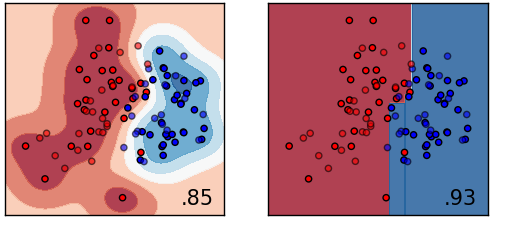
\includegraphics[width=7.5cm]{../pic/classification_example.png}\centering
	\end{center}
    \begin{block}{Замечание}
    Иногда для удобства fit возвращает не в диапазоне $[0, 1]$,
    а в диапазоне $[-1, 1]$.
    \end{block}
\end{frame}


 \begin{frame}
	 \begin{block}{Замечание}
	 	$U_{fit}$ в общем случае это именно неупорядоченная совокупность, а не множество. Во множестве ни один элемент не может быть более одного раза, а в неупорядоченной совокупности -- может. Для простоты в дальнейшем 	$U_{fit}$ будем называть множеством.
	 \end{block}
	\begin{block}{Замечание}
		Иногда функция $fit$ представляет собой \term{ленивое вычисление}\footnote{
		\termdef{Ленивые вычисления} (lazy evaluation, отложенные вычисления) -- 
		метод программной разработки функций, в которой вычисления откладывают до тех пор,
		пока не понадобится их результат.
		} и выдаёт $score$ почти мгновенно. И уже для каждого конкретного $\bold x$ функция
		$score(\bold x)$ рассчитывает \term{отклик} $\hat{y}$ на основании 
		\term{обучающей выборки} \term{} $U_{fit}$
	\end{block}
   \end{frame}
  
	\begin{frame}
	Без использования алгоритмов машинного обучения, функцию $score$ необходимо разрабатывать 
	<<вручную>>. Пример слайда №\ref{frame:class_feature_vector_example}:
	\begin{center}\small \begin{tabular}{ l l }
			$0 \mapsto (3234, 25, 1, 1731) $ &  $0 \mapsto (2540, 55, 0, 1731)$ \\
			$1 \mapsto (18400, 45, 0, 3137)$ & $0 \mapsto (2540, 55, 0, 1731)$  \\
			$1 \mapsto (903, 19, 0, 4121)$  & $0 \mapsto (1875, 45, 0, 4121)$  \\
			$0 \mapsto (854, 21, 1, 4121)$  & $1 \mapsto (702, 21, 0, 4121)$  \\
			$1 \mapsto (903, 19, 0, 4121)$  & $0 \mapsto (1875, 45, 0, 4121)$  \\
			$0 \mapsto (28400, 41, 1, 3137)$ & $0 \mapsto (25040, 55, 0, 1731)$  \\
	\end{tabular}\end{center}
	
	Можно задать функцию $score$ следующим способом:
	\begin{equation}\label{eq:score_example}
		score := \left\{ 
			\begin{array}
			[c]{ll}%
			0, ~$если$~ x_3 = 1 \vee x_4 = 1731
			\\
			0.6667, ~$если$~ x_3 = 0  \wedge x_4 \neq 1731
			\end{array}
		\right.
	\end{equation}

	\end{frame}

	\begin{frame}{Переобучение (Переподгонка, Overfitting)}
	\termdef{Переобучение} -- эффект построенной модели (функция $score$), 
	при котором на тестовой выборке модель работает существенно хуже.
	\begin{wrapfigure}{l}{0.4\textwidth}
	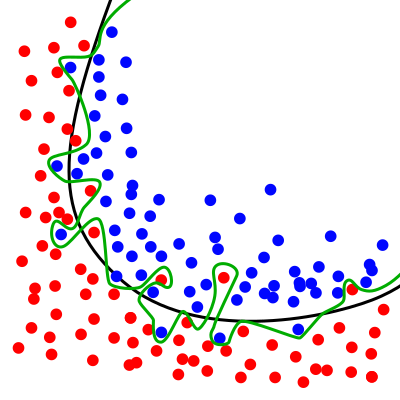
\includegraphics[width=4cm]{../pic/overfitting_example.png}\centering
	% \caption{Пример переобучения и нормального обучения}
	\end{wrapfigure}	
	Это связано с тем, что при построении модели («в процессе обучения») в обучающей выборке обнаруживаются некоторые случайные закономерности, которые отсутствуют в генеральной совокупности.
	\end{frame}
   	
   	\begin{frame}{Пример переобучения}
   	В примере \eqref{eq:score_example} у нас никогда не бывает мошенничества если клиент является 
   	мужчиной ($x_3=1$):
   	 \begin{equation*}
   	score := \left\{ 
   	\begin{array}
   	[c]{ll}%
   	0, ~$если$~ x_3 = 1 \vee x_4 = 1731
   	\\
   	0.6667, ~$если$~ x_3 = 0  \wedge x_4 \neq 1731
   	\end{array}
   	\right.
   	\end{equation*}
   	Однако это абсурд! Просто у нас такая выборка:
   \begin{center}\small \begin{tabular}{ l l }
   		$0 \mapsto (3234, 25, 1, 1731) $ &  $0 \mapsto (2540, 55, 0, 1731)$ \\
   		$1 \mapsto (18400, 45, 0, 3137)$ & $0 \mapsto (2540, 55, 0, 1731)$  \\
   		$1 \mapsto (903, 19, 0, 4121)$  & $0 \mapsto (1875, 45, 0, 4121)$  \\
   		$0 \mapsto (854, 21, 1, 4121)$  & $1 \mapsto (702, 21, 0, 4121)$  \\
   		$1 \mapsto (903, 19, 0, 4121)$  & $0 \mapsto (1875, 45, 0, 4121)$  \\
   		$0 \mapsto (28400, 41, 1, 3137)$ & $0 \mapsto (25040, 55, 0, 1731)$  \\
   \end{tabular}\end{center}
	\end{frame}
   
\begin{frame}{Обучение с подкреплением, reinforcement learning (Дообучение, Refitting)}
  	Есть первоначальная обучающая выборка: 
   \begin{equation*}
    U_{fit} = \left\{ y \mapsto \bold x  \right\}
   \end{equation*}
 	Первоначальное обучение:
  \begin{equation*}
  score_1 := fit (U_{fit}) 
  \end{equation*} 
  	В дальнейшем при получении нового множества $\hat U_{fit}$ (возможно состоящее из одного элемента)
  	мы дообучаем систему:
  	\begin{equation}
  	score_{i+1} := refit (\hat U_{fit}, score_{i}) 
  	\end{equation} 
   	Таким образом функция $score_i$ заменяется на новую функцию $score_{i+1}$.
\end{frame}

	\section{Тестовая выборка. Отсечка. tp, tn, fp, fn. Расчёт полноты и точность.}\label{section:precision_recall_defs}

	\begin{frame}
	Итак, у нас построена $score$ каким-либо алгоритмом машинного обучения. 
	Пока оставим за скобками как этот алгоритм построен. Это <<чёрный ящик>>.
		
	\begin{center}
	
\includegraphics[width=5cm]{../pic/magic_box.png}\centering
	\end{center}
	\end{frame}

	

	\begin{frame}{Тестовая выборка}
	После того как мы задали функцию оценщика ($score$)
	необходимо как-то оценить качество этой функции.
	
	Для этого мы выбираем другую выборку $U_{test}$ и для каждого $\bold x \in U_{test}$ 
	находим $\hat y$. 
	
	Таким образом можно задать совокупность пар:
	\begin{equation}
	\{(y, \hat y)\} := \left\{ (y, \hat y)~~\forall (\bold x, y) \in U_{test} : \hat y := score(\bold x) \right\} 
	\end{equation}
	
	После того, как мы задали какую либо отсечку ($offset$), мы каждую пару $(y, \hat y)$ можем отнести к одному из четырёх 
	событий: \textbf{true positive (tp), true negative (tn), false positive (fp), false negative (fn)}.
		
	\auditorium{Вспоминаем первую лекцию. Что такое полнота и точность?}
	\end{frame}

	\begin{frame}
	Просмотрим для определённой отсечки $offset$
	множество ${y, \hat y}$. 
	Если $\hat y \geqslant offset$ -- то это \textbf{positive}, 
	если $\hat y < offset$ -- то это \textbf{negative}.
	
	Если $y=0$ и \textbf{negative} или $y=1$ и \textbf{positive}, то это \textbf{true} negative/positive.
	Иначе \textbf{false}  negative/positive.
	
	Определим величины:
	\begin{enumerate}
		\item $ctp$ (count true positive) -- количество событий true positive (tp);
		\item $cfp$ (count false positive) -- количество событий false positive (fp);
		\item $ctn$ (count true negative) -- количество событий true positive (tn);
		\item $cfn$ (count false negative) -- количество событий false negative (fn).
	\end{enumerate}
	\end{frame}

	\begin{frame}{Вопрос на засыпку}
	Верно ли, что полноту ($\Pi$) и точность ($T$) можно определить с помощью формул?:
	\begin{equation*}
	\Pi = \frac{ctp}{ctp + cfn}
	\end{equation*}
	\begin{equation*}
	T = \frac{ctp}{ctp + cfp}
	\end{equation*}
	\auditorium{Мнение зала?}
	\end{frame}

	\begin{frame}{Вопрос на засыпку}
	Верно ли, что полноту ($\Pi$) и точность ($T$) можно определить с помощью формул?:
	\begin{equation*}
	\Pi = \frac{ctp}{ctp + cfn}
	\end{equation*}
	\begin{equation*}
	T = \frac{ctp}{ctp + cfp}
	\end{equation*}
	 \begin{block}{Запомните}
		Формула для полноты -- верна, а для точности -- нет!
	\end{block}
	\auditorium{Почему?}
	\end{frame}

	\begin{frame}{Вопрос на засыпку}
	Тестовая выборка $U_{test}$ является лишь подмножеством всех событий. 
	
	Как правило мошенничество составляет пренебрежимо малую часть всех транзакций в системе,
	поэтому за определённый промежуток времени для $U_{test}$ выбирают все события мошенничества.
	
	Однако взять и проскорить все легитимные операции физически невозможно.
	(Напрмер в Сбербанк Онлайне \textbf{ежесекундно} совершается в среднем 80 транзакций).
	Поэтому для $U_{test}$ выбирают лишь малую долю легитимных транзакций для проверки функции
	$score$.
	\end{frame}

	\begin{frame}{Полнота и точность}
	Введём величину $q_{legitim}$ -- это отношение количества легитимных транзакций во всей выборке, 
	делённая на количество легитимных транзакций в  $U_{test}$.
	
	Для любой отсечки $offset$ можем вычислить \termdef{полноту} ($\Pi$, recall) и \termdef{точность} ($T$, precision):
		\begin{equation}\label{eq:recall_by_counts}
		\Pi = \frac{ctp}{ctp + cfn}
		\end{equation}
		\begin{equation}\label{eq:presicionl_by_counts}
		T = \frac{ctp}{ctp + cfp \cdot q_{legitim}}
		\end{equation}
	\end{frame}



\section{Дерево решений. Лес решений}\label{section:tree_forest}

\begin{frame}
\begin{block}{Замечание}
	Алгоритмов машинного обучения очень много. 
	Хороший Data Scientist должен взять себе в привычку
	время от времени изучать те или иные алгоритмы.
	
	Цель курса -- прикладная. Научить решать ИБ задачи с помощью
	Data Science методов.
	
	Тем не менее хотя бы один алгоритм должен быть изучен.
\end{block}
\end{frame}

\begin{frame}{Дерево решений}
	Отрывок из <<Choosing the right estimator>>:\footnote{\tiny \url{https://scikit-learn.org/stable/tutorial/machine_learning_map/index.html}}
	\begin{center}
	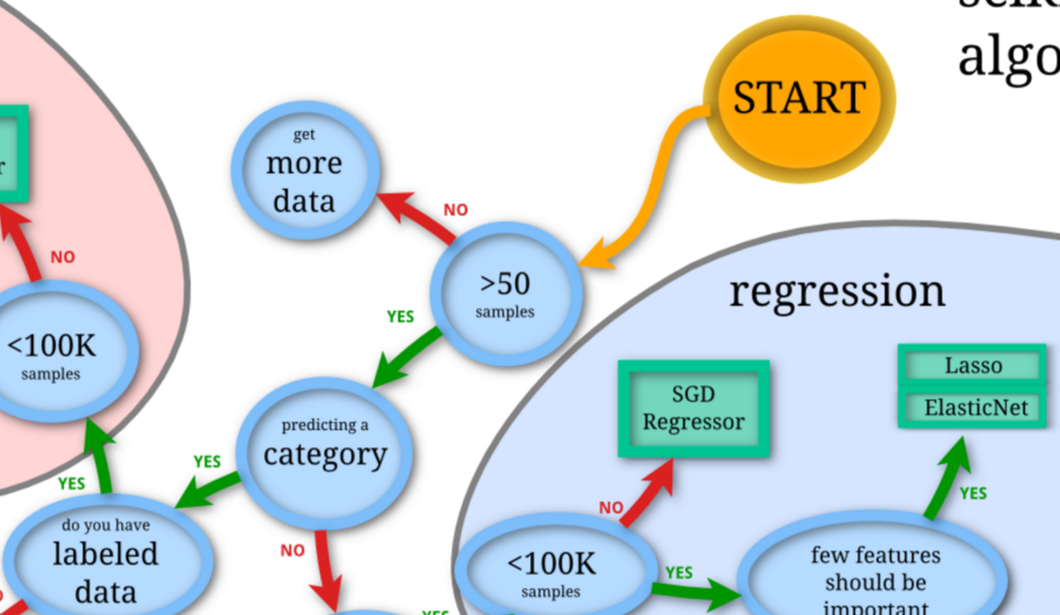
\includegraphics[width=6.5cm]{../pic/scikit_desicion_tree.png}\centering
	\end{center}
	На каждом шаге мы отвечаем на вопрос и "идем по дереву дальше".
\end{frame}

\begin{frame}{Пример дерева решений: <<Ирисы Фишера>>}
	\begin{center}
	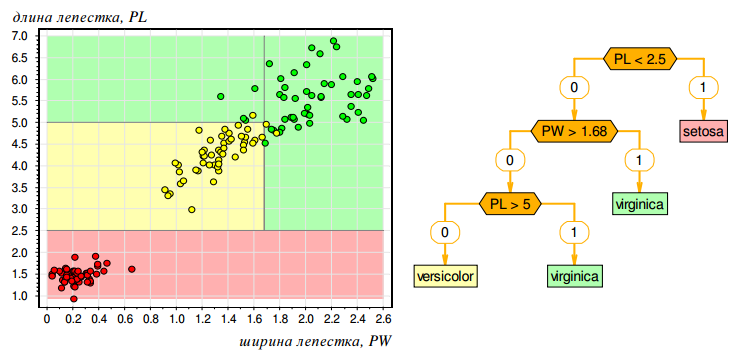
\includegraphics[width=11cm]{../pic/fisher_iris_tree.png}
	\end{center}
	Пример \term{экспертной системы}, являющийся решающим деревом.
\end{frame}

\begin{frame}{Пример дерева решений: <<Ирисы Фишера>>}
	\begin{center}
	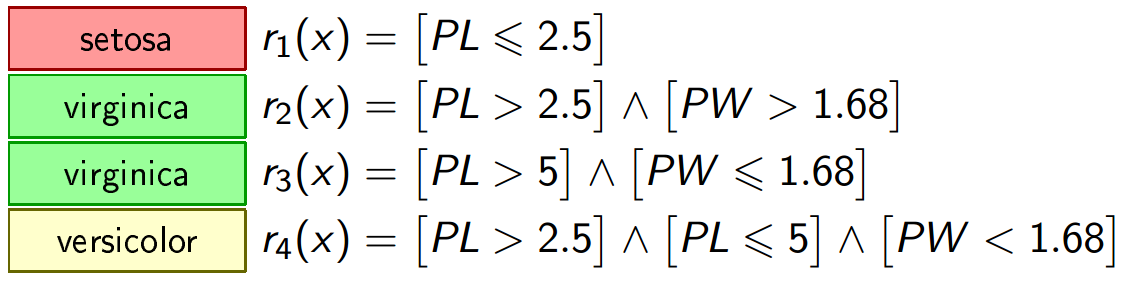
\includegraphics[width=11cm]{../pic/fisher_iris_boolean.png}
	\end{center}
	
	Любое \term{дерево решений} можно представить в виде совокупности
	булевых выражений.
\end{frame}

\begin{frame}{Формальное определение}
	\termdef{Дерево} -- это \fbox{связанный} \fbox{ациклический} \fbox{граф}
	имеющий выделенную вершину -- \fbox{корень} .
	
	\termdef{Дерево решений} -- это \fbox{дерево}, в терминальных вершинах которых 
	определён \term{отклик}, в остальных \fbox{узлах} -- функции\footnote{
	на практике -- \term{булевые} функции, но в общем определении -- не обязательно.}
	каждый выход из которых определяет метку какого-либо выходящего \fbox{ребра}.
\end{frame}

\begin{frame}{Лес решений.}
	\termdef{Лес решений} -- это \term{ансамбль}, каждый классификатор которого 
	является \term{деревом решений}.
	
	Обычно лес решений -- это среднее арифметическое всех его деревьев. 
	
	Например решаем задачу обнаружения мошенничества. Всего обучено 500 деревьев решений.
	На какой-либо транзакции 423 дерева определили что эта транзакция мошенническая,
	42 -- легитимная, остальные 35 деревьев -- отказ от классификации.
	
	\auditorium{Каков отклик данного леса?}
\end{frame}

\begin{frame}{Лес решений.}
	\termdef{Лес решений} -- это \term{ансамбль}, каждый классификатор которого 
	является \term{деревом решений}.
	
	Обычно лес решений -- это среднее арифметическое всех его деревьев. 
	
	Например решаем задачу обнаружения мошенничества. Всего обучено 500 деревьев решений.
	На какой-либо транзакции 423 дерева определили что эта транзакция мошенническая,
	42 -- легитимная, остальные 35 деревьев -- отказ от классификации.
	
	Тогда лес вернёт решение, что 
	с \term{априорной вероятностью}
	$p=\frac{423}{423+42} = 0.9097$ 
	данная операция является мошеннической.
\end{frame}

\begin{frame}
	\begin{block}{Замечание.}
	\small
	Лес решений -- это не обязательно среднее арифметическое \term{откликов}.
	\begin{equation}\label{eq:ensemble_p}
	p = \frac{1}{N} \cdot \sum_{i=1}^{N} \hat y_i
	\end{equation}
	где $\hat y = 1$, если подозрение на мошенничество или $\hat y =0$ иначе.
	
	Можно каждому $i$-му дереву  присвоить вес $w_i \geqslant 0$ и по разному его взвешивать:
	\begin{equation*}
	p = \frac{1}{ \sum_{i=1}^{N} w_i}  \cdot \sum_{i=1}^{N} \hat y_i \cdot w_i
	\end{equation*}
	Однако на практике в этом нет смысла.
	\end{block}

	\auditorium{Как изменится формула \eqref{eq:ensemble_p}, если добавить отклик <<отказ от классификации>>?}
\end{frame}

\section{Построение случайного дерева решений.}\label{section:random_tree_building}

\begin{frame}
	\begin{block}{Замечание}
	Существует большое количество оптимизаций и улучшений. 
	Данное описание построения показывает СУТЬ работы. 
	Желающие понять тему до конца могут ознакомится с академическими работами 
	по построению современных Random Forest систем.
	\end{block}
\end{frame}

\begin{frame}{Постановка задачи}
	Пока рассмотрим случай, в котором \term{вектор признаков} 
	состоит всего из двух величин: $(x_1, x_2)$.
	
	Таким образом \term{обучающая выборка} $U_{fit}$ имеет вид:
	\begin{equation}
	U_{fit} = \left\{ y \mapsto (x_1, x_2 )\right\}
	\end{equation}
	
	Тогда требуется определить 
	\term{функцию высшего порядка}
	$fit$, которая принимает на
	вход $U_{fit}$ а на выходе возвращает функцию $score$:
	\begin{equation}
	score := fit(U_{fit}) 
	\end{equation}
	
	\fbox{Функция $score$ -- это \term{дерево решений}.}
	
	На выходе $score$ возвращает $\hat{y} \in \{0, 1\}$:
	\begin{equation}
	\hat {y} := score(x_1, x_2)
	\end{equation}
\end{frame}

\begin{frame}{Визуализация данных}
	Для удобства обозначим $y=1$ (мошенничество) красным кругом, 
	$y=0$ (легитимная операция) -- синим квадратом.
	
	Так как у нас вектор признаков $\bold x$ состоит из двух признаков $(x_1, x_2)$, 
	то каждую пару 
	$y \mapsto \bold x$
	можно визуализировать на плоскости:
	\begin{center}
	\begin{tikzpicture}[scale=1.5]
	    \tikzstyle{F}=[circle,thick,fill=red,minimum size=1mm]
    \tikzstyle{L}=[rectangle,thick,fill=blue,minimum size=1mm]
   
    % Draw axes
    \draw [<->,thick] (0,2.3) node (yaxis) [above] {$x_2$}
        |- (4,0) node (xaxis) [right] {$x_1$};
    
    \node [F]  at (2, 1) {};
    \node [F]  at (1.8, 0.8) {};
    \node [F]  at (1.5, 0.5) {};
    \node [F]  at (1.7, 1.2) {};
    \node [F]  at (1.4, 1.5) {};
    \node [F]  at (1.2, 1) {};
    \node [F]  at (0.9, 0.3) {};
    \node [F]  at (0.3, 1.1) {};
    \node [F]  at (0.7, 0.9) {};
    \node [F]  at (0.4, 0.4) {};
    
    \node [L]  at (3.2, 1.1) {};
    \node [L]  at (2.2, 0.4) {};
    \node [L]  at (2.6, 0.6) {};
    \node [L]  at (2.3, 1.2) {};
    \node [L]  at (2.5, 1.4) {};
    \node [L]  at (2.0, 1.3) {};
    \node [L]  at (1.8, 1.8) {};
    \node [L]  at (1.6, 1.9) {};
    \node [L]  at (1.0, 1.6) {};
    \node [L]  at (0.7, 1.4) {};
    \node [L]  at (0.3, 1.6) {};
    \node [L]  at (0.6, 1.9) {};
    \node [L]  at (3.2, 0.5) {};
    \node [L]  at (3.5, 0.7) {};
    \node [L]  at (2.9, 1.3) {};
    \node [L]  at (2.8, 1.9) {};
    \node [L]  at (3.1, 1.2) {};
    \node [L]  at (3.3, 2.0) {};
    \node [L]  at (3.5, 1.1) {};
    
    
    % Выброс
    \node [F]  at (3.2, 1.6) {};
    
    % \coordinate (c) at (2, 1);
    % \fill[red] (c) circle (2pt);

    % \coordinate (c) at (1, 1);
    % \fill[red] (c) circle (2pt);
	\end{tikzpicture}
	\end{center}
\end{frame}

\begin{frame}{Выброс}
	\termdef{Выброс} -- объект обучающей выборки (пара $y \mapsto \bold x$),
	<<выделяющееся из общей выборки>>
	\begin{center}
	\begin{tikzpicture}[scale=1.5]
	    \tikzstyle{F}=[circle,thick,fill=red,minimum size=1mm]
    \tikzstyle{L}=[rectangle,thick,fill=blue,minimum size=1mm]
   
    % Draw axes
    \draw [<->,thick] (0,2.3) node (yaxis) [above] {$x_2$}
        |- (4,0) node (xaxis) [right] {$x_1$};
    
    \node [F]  at (2, 1) {};
    \node [F]  at (1.8, 0.8) {};
    \node [F]  at (1.5, 0.5) {};
    \node [F]  at (1.7, 1.2) {};
    \node [F]  at (1.4, 1.5) {};
    \node [F]  at (1.2, 1) {};
    \node [F]  at (0.9, 0.3) {};
    \node [F]  at (0.3, 1.1) {};
    \node [F]  at (0.7, 0.9) {};
    \node [F]  at (0.4, 0.4) {};
    
    \node [L]  at (3.2, 1.1) {};
    \node [L]  at (2.2, 0.4) {};
    \node [L]  at (2.6, 0.6) {};
    \node [L]  at (2.3, 1.2) {};
    \node [L]  at (2.5, 1.4) {};
    \node [L]  at (2.0, 1.3) {};
    \node [L]  at (1.8, 1.8) {};
    \node [L]  at (1.6, 1.9) {};
    \node [L]  at (1.0, 1.6) {};
    \node [L]  at (0.7, 1.4) {};
    \node [L]  at (0.3, 1.6) {};
    \node [L]  at (0.6, 1.9) {};
    \node [L]  at (3.2, 0.5) {};
    \node [L]  at (3.5, 0.7) {};
    \node [L]  at (2.9, 1.3) {};
    \node [L]  at (2.8, 1.9) {};
    \node [L]  at (3.1, 1.2) {};
    \node [L]  at (3.3, 2.0) {};
    \node [L]  at (3.5, 1.1) {};
    
    
    % Выброс
    \node [F]  at (3.2, 1.6) {};
    
    % \coordinate (c) at (2, 1);
    % \fill[red] (c) circle (2pt);

    % \coordinate (c) at (1, 1);
    % \fill[red] (c) circle (2pt);

\tikzstyle{outlier}=[circle,thick,draw=black,thick, dotted,minimum size=8mm]
\node [outlier]  at (3.2, 1.6) {};
	\end{tikzpicture}
	\end{center}

	\begin{block}{Замечание.}
	Строгого определения термина \term{выброс}, не существует.
	\end{block}
\end{frame}

\begin{frame}{Индекс Джини}
	\small
	Пусть $n$ -- это количество классов. 
	(В нашем примере $n=2$).
	
	Зафиксируем некое \term{замкнутое подпространство} признаков и назовём его 
	бином\footnote{от англ \textbf{bin [bɪn]} -- контейнер, емкость, бак, урна.}
	($bin$).
	
	Определим $\Delta_i$ -- доля объектов класса $i$ относительно всех объектов в данном бине:
	\begin{equation}
	\Delta_i \stackrel{def}{=} \frac{ \parallel \{y \mapsto \bold x : y = y_i \wedge \bold x \in bin \} \parallel}
	{
	\parallel \{y \mapsto \bold x :  \bold x \in bin \} \parallel
	}
	\end{equation}	
	\begin{center}  
	\begin{tikzpicture}[scale=1.5]
	    \tikzstyle{F}=[circle,thick,fill=red,minimum size=1mm]
    \tikzstyle{L}=[rectangle,thick,fill=blue,minimum size=1mm]
   
   \node [L] at (0.1, 0.2) {};
   \node [L] at (0.5, 0.5) {};
   \node [F] at (0.2, 0.7) {};
   \node [F] at (0.8, 0.8) {};
   \node [F] at (0.5, 0.2) {};
   
   \draw [thick, dotted] (0,0) -- (0,1);
   \draw [thick, dotted] (0,1) -- (1,1);
   \draw [thick, dotted] (1,1) -- (1,0);
   \draw [thick, dotted] (1,0) -- (0,0);
	\end{tikzpicture} 
	Пример:
	$\Delta_0 = \frac{2}{5}$; 
	$\Delta_1 = \frac{3}{5}$
	\end{center}

\end{frame}

\begin{frame}{Индекс Джини}
	\small
	\termdef{Индекс (загрязненности) Джини} (Gini impurity) 
	некоего бина $bin$ -- это величина, вычисленная по формуле:
	\begin{equation}
	\delta (bin)= 1 - \sum_{i=0}^{n-1} \Delta_i ^ 2
	\end{equation}
	
	
	\begin{center}
	Пример:
	\begin{tikzpicture}[scale=1.5]
	    \tikzstyle{F}=[circle,thick,fill=red,minimum size=1mm]
    \tikzstyle{L}=[rectangle,thick,fill=blue,minimum size=1mm]
   
   \node [L] at (0.1, 0.2) {};
   \node [L] at (0.5, 0.5) {};
   \node [F] at (0.2, 0.7) {};
   \node [F] at (0.8, 0.8) {};
   \node [F] at (0.5, 0.2) {};
   
   \draw [thick, dotted] (0,0) -- (0,1);
   \draw [thick, dotted] (0,1) -- (1,1);
   \draw [thick, dotted] (1,1) -- (1,0);
   \draw [thick, dotted] (1,0) -- (0,0);
	\end{tikzpicture} 
	\end{center}
	
	\begin{equation*}
	\delta (bin) = 1 - \left( \frac{2}{5}\right)^2 - \left( \frac{3}{5}\right)^2 = 
	1 - \frac{13}{25} = \frac{12}{25} 
	\end{equation*}
	
	
	\begin{block}{Замечание}
	Не путайте \term{Индекс Джини} и 
	\term{Коэфициент Джини}. Это разные понятия.
	\end{block}
\end{frame}


\begin{frame}{Альтернативы Индекса Джини}
	Более <<классическим>> критерием является 
	\termdef{(информационная) энтропия по Шеннону}:
	\begin{equation}
	H(bin) = - \sum_{i=0}^{n-1} \Delta_i \cdot log_n \Delta_i 
	\end{equation}
	Однако на практике её вычислять достаточно долго. 
	Индекс Джини, это <<математически кастрированная энтропия>>,
	дающая почти те же результаты за более быстрое время.
	\end{frame}
	
	
	
	
	\begin{frame}
	\footnotesize
	\textbf{Шаг 0.} Вручную определим критерий остановки: $\delta_{stop}$. На практике $\delta_{stop}=10^{-3}...10^{-6}$. В нашем примере пусть $\delta_{stop}=0.25$. 
	
	\textbf{Шаг 1.} Определим случайно один из признаков. Допустим это $x_1$. 
	Определим случайно величину на отрезке $x_1$. Пусть это некое $a_1$. 
	Начертим ось, перпендикулярную $x_1$ и проходящую через $(a_1, 0)$.
	\begin{center}
	\begin{tikzpicture}[scale=1.5]
	    \tikzstyle{F}=[circle,thick,fill=red,minimum size=1mm]
    \tikzstyle{L}=[rectangle,thick,fill=blue,minimum size=1mm]
   
    % Draw axes
    \draw [<->,thick] (0,2.3) node (yaxis) [above] {$x_2$}
        |- (4,0) node (xaxis) [right] {$x_1$};
    
    \node [F]  at (2, 1) {};
    \node [F]  at (1.8, 0.8) {};
    \node [F]  at (1.5, 0.5) {};
    \node [F]  at (1.7, 1.2) {};
    \node [F]  at (1.4, 1.5) {};
    \node [F]  at (1.2, 1) {};
    \node [F]  at (0.9, 0.3) {};
    \node [F]  at (0.3, 1.1) {};
    \node [F]  at (0.7, 0.9) {};
    \node [F]  at (0.4, 0.4) {};
    
    \node [L]  at (3.2, 1.1) {};
    \node [L]  at (2.2, 0.4) {};
    \node [L]  at (2.6, 0.6) {};
    \node [L]  at (2.3, 1.2) {};
    \node [L]  at (2.5, 1.4) {};
    \node [L]  at (2.0, 1.3) {};
    \node [L]  at (1.8, 1.8) {};
    \node [L]  at (1.6, 1.9) {};
    \node [L]  at (1.0, 1.6) {};
    \node [L]  at (0.7, 1.4) {};
    \node [L]  at (0.3, 1.6) {};
    \node [L]  at (0.6, 1.9) {};
    \node [L]  at (3.2, 0.5) {};
    \node [L]  at (3.5, 0.7) {};
    \node [L]  at (2.9, 1.3) {};
    \node [L]  at (2.8, 1.9) {};
    \node [L]  at (3.1, 1.2) {};
    \node [L]  at (3.3, 2.0) {};
    \node [L]  at (3.5, 1.1) {};
    
    
    % Выброс
    \node [F]  at (3.2, 1.6) {};
    
    % \coordinate (c) at (2, 1);
    % \fill[red] (c) circle (2pt);

    % \coordinate (c) at (1, 1);
    % \fill[red] (c) circle (2pt);

\draw [thick, dotted] (3,0) -- (3,2.5);
\node at (3,-0.2) {$a_1$};
	\end{tikzpicture}
	\end{center}
	Таким образом мы разбили простраство признаков
	$R^n=R^2$ на два \term{бина}:
	\begin{enumerate}
	\item $r(x_1=a_1)$ -- бин, для которого $x_1 \geqslant a_1$;
	\item $l(x_1=a_1)$ -- бин для которого $x_1 < a_1$.
	\end{enumerate}
\end{frame}

\begin{frame}
	\small
	Посчитаем индекс Джини для каждого бина и сравним его с $\delta_{stop}$:
	\begin{center}
	\begin{tikzpicture}[scale=1.5]
	    \tikzstyle{F}=[circle,thick,fill=red,minimum size=1mm]
    \tikzstyle{L}=[rectangle,thick,fill=blue,minimum size=1mm]
   
    % Draw axes
    \draw [<->,thick] (0,2.3) node (yaxis) [above] {$x_2$}
        |- (4,0) node (xaxis) [right] {$x_1$};
    
    \node [F]  at (2, 1) {};
    \node [F]  at (1.8, 0.8) {};
    \node [F]  at (1.5, 0.5) {};
    \node [F]  at (1.7, 1.2) {};
    \node [F]  at (1.4, 1.5) {};
    \node [F]  at (1.2, 1) {};
    \node [F]  at (0.9, 0.3) {};
    \node [F]  at (0.3, 1.1) {};
    \node [F]  at (0.7, 0.9) {};
    \node [F]  at (0.4, 0.4) {};
    
    \node [L]  at (3.2, 1.1) {};
    \node [L]  at (2.2, 0.4) {};
    \node [L]  at (2.6, 0.6) {};
    \node [L]  at (2.3, 1.2) {};
    \node [L]  at (2.5, 1.4) {};
    \node [L]  at (2.0, 1.3) {};
    \node [L]  at (1.8, 1.8) {};
    \node [L]  at (1.6, 1.9) {};
    \node [L]  at (1.0, 1.6) {};
    \node [L]  at (0.7, 1.4) {};
    \node [L]  at (0.3, 1.6) {};
    \node [L]  at (0.6, 1.9) {};
    \node [L]  at (3.2, 0.5) {};
    \node [L]  at (3.5, 0.7) {};
    \node [L]  at (2.9, 1.3) {};
    \node [L]  at (2.8, 1.9) {};
    \node [L]  at (3.1, 1.2) {};
    \node [L]  at (3.3, 2.0) {};
    \node [L]  at (3.5, 1.1) {};
    
    
    % Выброс
    \node [F]  at (3.2, 1.6) {};
    
    % \coordinate (c) at (2, 1);
    % \fill[red] (c) circle (2pt);

    % \coordinate (c) at (1, 1);
    % \fill[red] (c) circle (2pt);

\draw [thick, dotted] (3,0) -- (3,2.5);
\node at (3,-0.2) {$a_1$};
	\end{tikzpicture}
	\end{center}
	\begin{equation*}
	\delta \left(r(x_1=a_1)\right) = 
	1 - \left(\frac{6}{7}\right)^2 - \left( \frac{1}{7}\right)^2 =
	\frac{12}{49} \leqslant 0.25 = \delta_{stop}
	\end{equation*}
	\begin{equation*}
	\delta \left(l(x_1=a_1)\right) = 
	1 - \left( \frac{13}{23} \right)^2 - \left( \frac{10}{23} \right)^2 
	= \frac{260}{529} \approx 0,49149 > 0.25 = \delta_{stop}
	\end{equation*}
	Если индекс Джини не больше $\delta_{stop}$, то в рамках данного бина выносим 
	вердикт (отклик). Иначе повторяем шаг 1, в рамках выбранного бина.
\end{frame}

\begin{frame}{Пересечение бинов}
	Определим операцию $bin_1 \cap bin_2$ -- означающую пересечение бинов.
	
	Например:
	\begin{equation*}
	r(x_1=a_1)  \cap r(x_2=a_2) \cap l(x_1=a_3)
	\end{equation*}
	Означает:
	\begin{equation*}
	\begin{cases}
	x_1 \geqslant  a_1 \\
	x_2 \geqslant a_2 \\
	x_1 < a_3 \\
	\end{cases}
	\end{equation*}
\end{frame}

\begin{frame}
	\small
	\textbf{Шаг 2.} Допустим что теперь случайным образом выбрали $x_2$.
	Определили $a_2$.
	\begin{center}
	\begin{tikzpicture}[scale=1.5]
	    \tikzstyle{F}=[circle,thick,fill=red,minimum size=1mm]
    \tikzstyle{L}=[rectangle,thick,fill=blue,minimum size=1mm]
   
    % Draw axes
    \draw [<->,thick] (0,2.3) node (yaxis) [above] {$x_2$}
        |- (4,0) node (xaxis) [right] {$x_1$};
    
    \node [F]  at (2, 1) {};
    \node [F]  at (1.8, 0.8) {};
    \node [F]  at (1.5, 0.5) {};
    \node [F]  at (1.7, 1.2) {};
    \node [F]  at (1.4, 1.5) {};
    \node [F]  at (1.2, 1) {};
    \node [F]  at (0.9, 0.3) {};
    \node [F]  at (0.3, 1.1) {};
    \node [F]  at (0.7, 0.9) {};
    \node [F]  at (0.4, 0.4) {};
    
    \node [L]  at (3.2, 1.1) {};
    \node [L]  at (2.2, 0.4) {};
    \node [L]  at (2.6, 0.6) {};
    \node [L]  at (2.3, 1.2) {};
    \node [L]  at (2.5, 1.4) {};
    \node [L]  at (2.0, 1.3) {};
    \node [L]  at (1.8, 1.8) {};
    \node [L]  at (1.6, 1.9) {};
    \node [L]  at (1.0, 1.6) {};
    \node [L]  at (0.7, 1.4) {};
    \node [L]  at (0.3, 1.6) {};
    \node [L]  at (0.6, 1.9) {};
    \node [L]  at (3.2, 0.5) {};
    \node [L]  at (3.5, 0.7) {};
    \node [L]  at (2.9, 1.3) {};
    \node [L]  at (2.8, 1.9) {};
    \node [L]  at (3.1, 1.2) {};
    \node [L]  at (3.3, 2.0) {};
    \node [L]  at (3.5, 1.1) {};
    
    
    % Выброс
    \node [F]  at (3.2, 1.6) {};
    
    % \coordinate (c) at (2, 1);
    % \fill[red] (c) circle (2pt);

    % \coordinate (c) at (1, 1);
    % \fill[red] (c) circle (2pt);

\draw [thick, dotted] (3,0) -- (3,2.5);
\node at (3,-0.2) {$a_1$};

\draw [thick, dotted] (0,0.9) -- (3,0.9);
\node at (-0.15,1-0.1) {$a_2$};
	\end{tikzpicture}
	\end{center}
	\begin{equation*}
	\delta \big(l(x_1=a_1) \cap r(x_2=a_2)\big) = 
	1 - \left( \frac{11}{17} \right)^2 - \left( \frac{6}{17} \right)^2
	= \frac{132}{289} \approx 0,4567 > 0.25
	\end{equation*}
	\begin{equation*}
	\delta \big(l(x_1=a_1) \cap l(x_2=a_2)\big) = 
	1 - \left( \frac{2}{6} \right)^2  - \left( \frac{4}{6} \right)^2  
	= \frac{16}{36} \approx 0.4444 > 0.25
	\end{equation*}
	Вывод: в обоих бинах строим дерево решений дальше. Нет остановки.
\end{frame}

\begin{frame}
	\small
	\textbf{Шаг 3}.
	В бине $\big(l(x_1=a_1) \cap r(x_2=a_2)\big)$
	случайно выбрали $x_2$ и $a_3$.
	
	В бине $ \big(l(x_1=a_1) \cap l(x_2=a_2)\big)$
	случайно выбрали $x_1$ и $a_4$.
	
	\begin{center}
	\begin{tikzpicture}[scale=1.5]
	\input{./../pic/desicion_tree_building/1.tikz.tex}

\draw [thick, dotted] (3,0) -- (3,2.5);
\node at (3,-0.2) {$a_1$};

\draw [thick, dotted] (0,0.9) -- (3,0.9);
\node at (-0.15,1-0.1) {$a_2$};

\draw [thick, dotted] (0,1.6) -- (3,1.6);
\node at (-0.15,1.6-0.1) {$a_3$};

\draw [thick, dotted] (2.1,0) -- (2.1, 0.9);
\node at (2.1,-0.2) {$a_4$};
	\end{tikzpicture}
	\end{center}
	Очень удачный шаг. 
	Остался бин $l(x_1=a_1) \cap r(x_2=a_2) \cap l(x_2=a_3)$.
\end{frame}

\begin{frame}
	\small
	\textbf{Шаг 4}.
	\begin{center}
	\begin{tikzpicture}[scale=1.5]
	\input{./../pic/desicion_tree_building/2.tikz.tex}

\draw [thick, dotted] (0,0.9) -- (3,0.9);
\node at (-0.15,1-0.1) {$a_2$};

\draw [thick, dotted] (0,1.6) -- (3,1.6);
\node at (-0.15,1.6-0.1) {$a_3$};

\draw [thick, dotted] (2.1,0) -- (2.1, 0.9);
\node at (2.1,-0.2) {$a_4$};


\draw [thick, dotted] (2.0,0.9) -- (2.0, 1.6);
\node at (2.1-0.15,0.9-0.2-0.1) {$a_5$};
	\end{tikzpicture}
	\end{center}
	Конец алгоритма. Индекс Джини всех бинов не больше чем $\delta_{stop}$.
	\begin{block}{Замечание}
	Данное дерево было построено случайным образом. 
	При повторном запуске алгоритма может получится другое дерево.
	\end{block}
\end{frame}

\begin{frame}{Случайное дерево решений.}
	\small
	Случайное дерево решений -- это 
	\term{бинарный} классификатор,
	возвращающий априорную вероятность:
	\begin{itemize}
	\item $p=0$ -- легитимная операция
	\item $p=1$ -- мошенническая операция
	\end{itemize}

	\begin{wrapfigure}{l}{0.65\textwidth}
	\vspace{-25pt}
	\begin{tikzpicture}[scale=1.5]
	\input{./../pic/desicion_tree_building/3.tikz.tex}

\draw [thick, dotted] (0,1.6) -- (3,1.6);
\node at (-0.15,1.6-0.1) {$a_3$};

\draw [thick, dotted] (2.1,0) -- (2.1, 0.9);
\node at (2.1,-0.2) {$a_4$};


\draw [thick, dotted] (2.0,0.9) -- (2.0, 1.6);
\node at (2.1-0.15,0.9-0.2-0.1) {$a_5$};

\tikzstyle{zone1}=[semitransparent,dashed,thick,draw=black,fill=red!20]
\tikzstyle{zone0}=[semitransparent,dashed,thick,draw=black,fill=blue!20]

\draw [zone0] (0+0.05,1.6+0.05) rectangle (3-0.05,2.3);
\draw [zone1] (0+0.05,0.9+0.05) rectangle (2.0-0.05,1.6-0.05);
\draw [zone1] (0+0.05,0.0+0.05) rectangle (2.1-0.05,0.9-0.05);
\draw [zone0] (2.0+0.05,0.9+0.05) rectangle (3-0.05,1.6-0.05);
\draw [zone0] (2.1+0.05,0.0+0.05) rectangle (3-0.05,0.9-0.05);
\draw [zone0] (3+0.05,0.0+0.05) rectangle (3.9,2.3);
	\end{tikzpicture}
	\end{wrapfigure}
	
	На рисунке бины, для которых $p=0$ отмечены голубыми областями,
	а бины, для которых $p=1$ отмечены красными областями.
	
\end{frame}

\begin{frame}{Точки остановки}
	Помимо \term{индекса Джини} (параметр $min\_impurity\_split$ в scikit-learn)
	можно использовать другие точки остановки:
	\begin{itemize}
	\item Количество данных (векторов признаков)
	в бине меньше $min\_samples\_split$;
	\item Глубина дерева достигла $max\_depth$.
	\end{itemize}
	
	\auditorium{ДЗ. Посмотреть: \url{https://scikit-learn.org/stable/modules/generated/sklearn.ensemble.RandomForestClassifier}}
\end{frame}

\section{Случайный Лес (Random Forest)}\label{section:random_forest}

\begin{frame}
	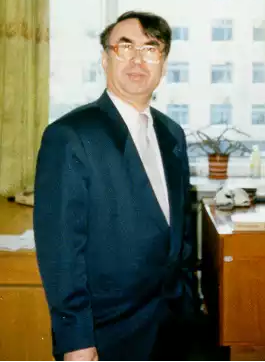
\includegraphics[width=4.5cm]{../pic/ylpavlov.png}
	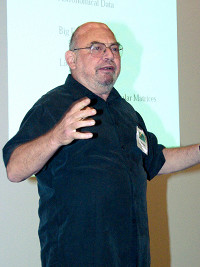
\includegraphics[width=4.5cm]{../pic/leo_breiman.png}
	Изобретатели Случайного Леса (Random Forest):
	\begin{itemize}
	\item Павлов Юрий Леонидович (р.1949)
	\item Лео Брейнман (Leo Breiman) (1928 — 2005)
	\end{itemize}
\end{frame}

\begin{frame}
	\termdef{Случайный лес} -- это \term{ансамбль}
	случайных деревьев (на практике от 100 до 1000).
	
	В общем случае случайным образом выбираются:
	\begin{enumerate}
	\item подмножество признаков, на котором строим дерево
	\item подмножество обучающей выборки
	\item выбор признака и значения разбиения.
	\end{enumerate}	
\end{frame}

\begin{frame}
	Обычно берут функцию голосования. 
	Всего $N$ деревьев, 
	$n_1$ -- количество деревьев вернувших 1,
	$n_0$ -- количество деревьев, вернувших 0,
	при этом $n_0 + n_1 \leqslant N$. 
	(Если нет отказа от классификации, то $n_0 + n_1 = N$).
	
	Тогда \term{априорная вероятность} мошенничества
	вычисляется по формуле:
	\begin{equation}
	p = \frac{n_1}{n_1+n_0}
	\end{equation}
	
	\begin{block}{Замечание.}
	Вместо функции голосования, можно брать любое другое 
	\textbf{среднее по Колмогорову} или другую функцию.
	\end{block}
\end{frame}

\begin{frame}{<<Центральная эмпирическая <<теорема>> о Случайном Лесе>>}
	\begin{block}{<<Ц.Э.Т>>}
	<<Если вы работаете в области,
	в которой совершенно некомпетентны
	и/или решаете задачу, про которую ничего не знаете --
	используйте случайный лес.
	Этот алгоритм М.О. -- самый лучший!>>
	\end{block}
	Это совершенно <<не академично>>, но истинно.
	
	Более того, т.к. в задачах ИБ, ваш противник --
	человек, то следует все усилия приложить на 
	Feature Extraction, а в качестве алгоритма М.О.
	использовать Random Forest. 
\end{frame}

\begin{frame}{Выводы <<Ц.Э.Т.>>}
	Выводы: 
	\begin{enumerate}
	\item Случайный лес -- решение многих 
	задач на вполне приемлемом уровне
	\item Сравните свой классификатор со случайным лесом 
	и вы поймете насколько ваш классификатор хорош
	\item По настоящему интересные задачи -- это те,
	которые не решаются случайным лесом.
	\end{enumerate}
\end{frame}

\begin{frame}{Достоинства RF}
	\footnotesize
	\begin{enumerate}
		\item очень просто устроен
		\item устойчивость к переобучению. 
		\item понятные и легко настраиваемые параметры
		\item либо RF работает, либо данные <<сырые>> и требуют предобработки (например выбор паттернов в изображении нейронной сетью)
		\item уже реализован. Легко программируем с нуля (для прошивок)
		\item быстрый. (Условия дерева решений if-then-else просты и быстрые.)
		\item $\sim$масштабируемый.
		\item RF является мощным средством против <<активного противника>>\footnote{
			в задачах с обратной связью изучаемого субъекта (хакера, мошенника)
		}. 
		\item не требует определения расстояния Махаланобиса\footnote{на след.лекциях будет}
	\end{enumerate}
\end{frame}

\section{Список материалов}

\begin{frame}{Случайные леса}
	Сергей Павлович Чистяков \href{http://resources.krc.karelia.ru/transactions/doc/trudy2013/trudy_2013_1_117-136.pdf}{<<Случайные леса: обзор>>}
	
	А.Дьяконов 
	\href{https://dyakonov.org/2016/11/14/\%D1\%81\%D0\%BB\%D1\%83\%D1\%87\%D0\%B0\%D0\%B9\%D0\%BD\%D1\%8B\%D0\%B9-\%D0\%BB\%D0\%B5\%D1\%81-random-forest/}{<<Случайный лес (Random Forest)>>}
	
	\textbf{sklearn}:
	\begin{itemize}
	\item \href{https://scikit-learn.org/stable/modules/generated/sklearn.ensemble.RandomForestClassifier.html}{sklearn.ensemble.RandomForestClassifier}
	\item \href{https://scikit-learn.org/stable/modules/generated/sklearn.ensemble.RandomForestRegressor.html}{sklearn.ensemble.RandomForestRegressor}
	\item \href{https://scikit-learn.org/stable/modules/generated/sklearn.ensemble.IsolationForest.html}{sklearn.ensemble.IsolationForest}
	\end{itemize}
\end{frame}

\begin{frame}{Support Vector Machines}
	
	Для любителей математики only.

	Попробуйте самостоятельно понять, как работает SVM.
	
	Из академических работ рекомендую Алексея Нефёдорова
	\href{https://svmtutorial.online}{<<Support Vector Machines: A Simple Tutorial>>}
	
\end{frame}

\section{Вопросы для самопроверки}

   \begin{frame}{Признаки, вектор признаков, выборка}
   \begin{enumerate}
   	\item Что такое \term{признак}?
   	\item Что такое несравнимый (категориальный) признак? Чем он отличается от сравнимого?
   	\item Что такое булев признак? Числовой?
   	\item Приведите пример булевого и несравнимого признака. Булевого и сравнимого. 
   	\item Что такое \term{вектор признаков}? Есть два вектора $\bold x_a = (x_1, x_2)$ и $\bold x_b = (x_2, x_1)$.
   	Являются ли они идентичными? Можете привести задачу, когда являются?
   	\item Что такое \term{обучающая выборка}? Почему формула \eqref{eq:def_fit_sample} задаётся
   	как \textbf{неупорядоченная} совокупность, а не как список (т.е. упорядоченная совокупность).
   	Почему порядок перечесления данных в аргументе функции \eqref{eq:fit_def} не важен?
   \end{enumerate}
	\end{frame}

\begin{frame}{Обучающая выборка со слайда №\ref{frame:class_feature_vector_example}}
 	Посмотрите на \term{выборку} со слайда №\ref{frame:class_feature_vector_example}. 
 	\begin{enumerate}
 	\item Верно ли утверждение, что если совершается оплата электроэнергии, то данная операция всегда легитимная?
 	\item Есть ли корреляция между возрастом клиента и мошенничеством при покупке авиабилетов? 
 	\item Можно ли предположить, что таксисты чаще обманывают молодых девушек? 
 	\item Покупает ли молодёжь авиабилеты через данный банк? 
 	\item Если совершают мошенничество в сфере автоперевозок, то обманывают мужчин или женщин?
	\end{enumerate}
	\end{frame}
  
  	\begin{frame}{Обучение и переобучение}
  		\begin{enumerate}
  			\item Что такое обучение (fitting)? Что такое переобучение? (overfitting)?
  			\item Почему функции $fit$ и $refit$ -- это функции высшего порядка?
  			\item Как с помощью ансамблирования уменьшить проблему переобучения (а для некоторых алгоритмов и вовсе его убрать) ?
  			\item можете предложить какую-либо меру измерить переобучение?
  			\item Верно ли утверждение, что чем больше и <<разнообразней>> выборка, тем меньше ошибок, вызванных переобучением?
  		\end{enumerate} 
	\end{frame}
  	
 \begin{frame}{Полнота, точность и $q_{fraud}$}
 		Существуют задачи, в которых физически невозможно рассчитать скоринг для всех 
 		мошеннических операций на определённом достаточном для анализа качества системы промежутке времени (например неделя).
 		К примеру -- это задача распознавания спама. Спама очень много...
 		
 		Тогда, для расчёта $\{y, \hat y\}$ выбирается лишь подмножество мошеннических операций для выборки $U_{test}$.
 		
 		Таким образом, аналогично $q_{legitim}$ разумно определить коэффициент $q_{fraud}$.
 		
 		Как тогда изменятся формулы \eqref{eq:recall_by_counts} и \eqref{eq:presicionl_by_counts}?
 \end{frame}
  
  
 \begin{frame}
  В банковской системе <<ВашБанк Онлайн>> введена система фрод-мониторинга. 
  Она представляет собой лес решений из 700 деревьев решений. Функция принятия решений -- среднее арифметическое. На определённой транзакции 573 деревьев определило транзакцию как мошенническую, 57 как легитимную, остальные -- отказ от классификации.
  \begin{enumerate}
  	\item каков отклик системы ФМ?
  	\item каков отклик системы ФМ, если отказ от классификации считать легитимными операциями?
  	\item каков отклик системы ФМ, если отказ от классификации считать подозрением на мошенничество?
  	\item каков отклик системы ФМ, если отказ от классификации считать подозрением на мошенничество, однако вклад брать не как 1, а как 0.7 ?
  \end{enumerate}
  
\end{frame}


\begin{frame}{Индекс Джини и бины}
	\begin{enumerate}
	\item Почему на практике используют индекс Джини, а не энтропию по Шеннону? 
	Можете придумать ещё более простую <<меру загрязнённости>>, чем индекс Джини?
	\item При каких условиях индекс Джини равен нулю? При каких 1/2 ? 
	При каких равен 1? При каких условиях не определён?
	\item Докажите что для любого количества классов $n$, индекс Джини лежит в границах: $\delta \in [0, \frac{1}{2}]$.
	\item Почему бины обязательно квадратные, а не круглые или треугольные? Какая разница
	в каком подпространстве признаков рассчитывать индекс Джини? 	
	\end{enumerate}
\end{frame}



\begin{frame}{Случайное дерево. Случайный лес.}
	\begin{enumerate}
	\item С помощью кванторов и слов 
	напишите строгий академический алгоритм,
	описывающий построение случайного дерева 
	над пространством признаков $R^n$.
	\item Аналогично п.1, напишите 
	строгий академический алгоритм,
	описывающий построение случайного леса
	\item Объясните, почему RF устойчив к переобучению.
	\item Объясните, почему RF очень легко реализуем на ПЛИС.
	\item Пусть есть некий признак $x_i$ принимающий одно из значений: 
	<<русский>>, <<француз>>, <<чукча>>, <<арапеш>>. Как задать функции
	$r\big(x_i=a\big)$ и $l\big(x_i=a\big)$ ? 
	\item В RF количество деревьев $N$ -- параметр. 
	Придумайте алгоритм автоматического\footnote{=без участния эксперта} нахождения оптимального $N$
	для любой обучающей выборки.
	\end{enumerate} 
\end{frame} 

\end{document}